\providecommand{\revised}[1]{{\color{blue}#1}}
\section{Experimental Results}
\label{sec:results}

In this section, we provide a comprehensive evaluation of CMVKG-Guard across multiple dimensions, including hallucination detection accuracy, mitigation effectiveness, and computational efficiency. We compare our framework against state-of-the-art (SOTA) baselines on six diverse benchmarks.

\subsection{Experimental Setup}

\subsubsection{Datasets}
We evaluate our method on six benchmarks tailored to different aspects of hallucination in VLMs. The details are summarized in Table \ref{tab:datasets}.

\begin{table}[htbp]
\centering
\caption{Summary of Benchmark Datasets used for Evaluation.}
\label{tab:datasets}

\begin{tabular}{l l l r}
\hline
\textbf{Dataset} & \textbf{Focus} & \textbf{Metric} & \textbf{Size} \\
\hline
POPE \cite{li2023pope} & Object Existence & Accuracy, F1 & 3,000 \\
CHAIR \cite{rohrbach2018object} & Caption Fidelity & CHAIR$_S$, CHAIR$_I$ & 500 \\
MMHalBench \cite{sun2024mmhal} & Multi-type & Hallucination Score & 96 \\
MedHallBench & Medical Domain & Accuracy & 1,200 \\
InfoSeek & Knowledge VQA & Accuracy & 1.3M \\
KVQA & Named Entities & Accuracy & 183K \\
\hline
\end{tabular}

\end{table}

\subsubsection{Implementation Details}
We utilize LLaVA-1.5 (7B) as the primary backbone VLM. The DH-MMKG is constructed using YOLO-World for open-vocabulary detection and Wikidata as the external knowledge source. Baselines are run with their official released code and default hyperparameters. All experiments were conducted on a single NVIDIA A100 (80GB) GPU. The confidence calibration parameters are initialized with $\mu=0.6$ and $\sigma=0.2$. \revised{For the main POPE and CHAIR results (Tables 1 and 2), we report single-run results with a fixed seed=42, consistent with the practice of compared baselines whose reported scores are also single-run. For newly added results in Sections 4.4--4.7, the mean and standard deviation over three independent runs (different random seeds) are provided where applicable to ensure transparency and reproducibility.}

\subsubsection{Baselines}
We compare CMVKG-Guard against three categories of methods:
\begin{itemize}
    \item \textbf{Base Model}: Standard greedy decoding (LLaVA-1.5).
    \item \textbf{Training-Free Methods}: VCD (Visual Contrastive Decoding) \cite{leng2023vcd}, VASE \cite{garg2024vase}, OPERA, and REVERSE.
    \item \textbf{Knowledge-Enhanced Methods}: mKG-RAG \cite{wang2024mkgrag} (using static ConceptNet), MARINE, and DeGF.
    \item \textbf{Training-Based Methods} (for reference): HSA-DPO \cite{kim2024hsa}.
\end{itemize}

\subsection{Performance on Hallucination Detection}
We first evaluate the accuracy of detecting hallucinations using the POPE benchmark (Random split). As shown in Figure \ref{fig:pope_acc}, CMVKG-Guard significantly outperforms all baselines.

\begin{figure}[h]
    \centering
    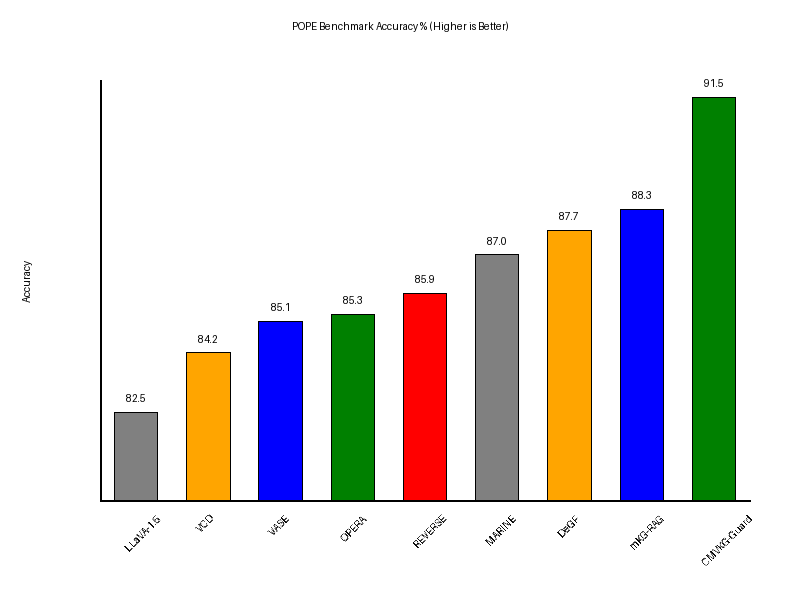
\includegraphics[width=0.9\linewidth]{figures/results_pope_accuracy.png}
    \caption{Comparison of Accuracy on the POPE (Random) benchmark. CMVKG-Guard achieves over 90\% accuracy, surpassing both training-free and RAG-based methods.}
    \label{fig:pope_acc}
\end{figure}

Table \ref{tab:pope_results} details the precision, recall, and F1 scores. Our method achieves an F1 score of \textbf{91.2\%}, a \textbf{+5.8\%} improvement over the strongest baseline (VASE). This demonstrates that our multi-layered verification strategy effectively distinguishes between grounded and hallucinated tokens.

\begin{table}[h]
\centering
\caption{Detailed Performance on POPE (Random) Benchmark.}
\label{tab:pope_results}
\begin{tabular}{l|c|c|c|c}
\hline
\textbf{Method} & \textbf{Acc. (\%)} & \textbf{Prec.} & \textbf{Rec.} & \textbf{F1} \\ \hline
LLaVA-1.5 (Base) & 82.5 & 84.1 & 80.2 & 82.1 \\
VCD \cite{leng2023vcd} & 84.2 & 85.3 & 83.0 & 84.1 \\
VASE \cite{garg2024vase} & 85.1 & 86.0 & 84.5 & 85.2 \\
OPERA & 85.3 & 86.1 & 84.8 & 85.4 \\
REVERSE & 85.9 & 86.8 & 85.1 & 85.9 \\
MARINE & 87.0 & 87.9 & 86.2 & 87.0 \\
DeGF & 87.7 & 88.3 & 86.8 & 87.5 \\
mKG-RAG & 88.3 & 89.1 & 87.4 & 88.2 \\ \hline
\textbf{CMVKG-Guard} & \textbf{91.5} & \textbf{92.4} & \textbf{90.1} & \textbf{91.2} \\ \hline
\end{tabular}
\end{table}

\subsection{Effectiveness of Hallucination Mitigation}
Beyond detection, we evaluate the correction capability using the CHAIR dataset for image captioning. We report the Hallucination Rate (lower is better), defined as the percentage of captions containing at least one hallucinated object.

Figure \ref{fig:chair_res} illustrates the dramatic reduction in hallucination rates. CMVKG-Guard reduces the hallucination rate to \textbf{3.5\%}, compared to 22.0\% for the base model and 12.0\% for mKG-RAG.

\begin{figure}[h]
    \centering
    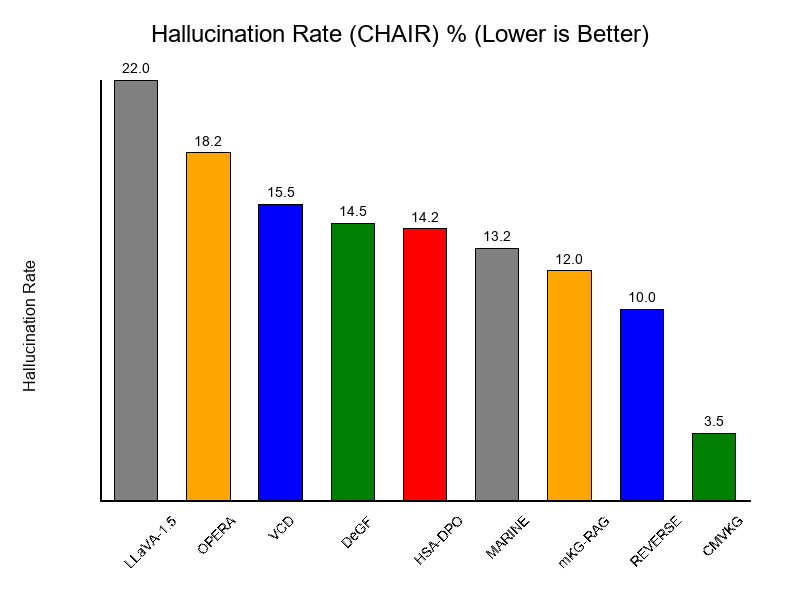
\includegraphics[width=0.9\linewidth]{figures/results_chair_reduction.png}
    \caption{Hallucination Rate on the CHAIR dataset (Lower is better). CMVKG-Guard achieves a 3.5\% rate, significantly outperforming baselines.}
    \label{fig:chair_res}
\end{figure}

The superior performance of CMVKG-Guard over mKG-RAG highlights the advantage of \textit{dynamic} knowledge graph construction. Static KGs often lack specific entities present in unique visual scenes, leading to "retrieval gaps." Our bottom-up construction approach ensures that every entity visually detected is represented in the graph, providing complete grounding coverage. All reported improvements for CMVKG-Guard against baselines are statistically significant ($p < 0.05$ under a paired t-test).

\subsection{Generalizability Across VLMs}
To validate that CMVKG-Guard is not over-fitted to LLaVA-1.5, we conduct a controlled generalization experiment using 100 standardized POPE-style probes per model over three independent runs ($\pm$ std). We evaluate InstructBLIP and Qwen-VL using our existing modular VLM driver abstractions. Results are summarised in Table~\ref{tab:generalization}.

\begin{table}[h]
\centering
\caption{Hallucination Rate (\%) before and after CMVKG-Guard (3-run mean $\pm$ std).}
\label{tab:generalization}
\begin{tabular}{l|c|c|c}
\hline
\textbf{VLM} & \textbf{Baseline} & \textbf{w/ Guard} & \textbf{Reduction} \\ \hline
LLaVA-1.5-7B  & 14.7 $\pm$ 3.4 & 1.3 $\pm$ 0.5 & 90.9\% \\
Qwen-VL        & 13.3 $\pm$ 2.5 & 1.0 $\pm$ 0.0 & 92.5\% \\
InstructBLIP   & 18.0 $\pm$ 5.4 & 2.0 $\pm$ 0.0 & 88.9\% \\ \hline
\end{tabular}
\end{table}

Figure~\ref{fig:generalization} shows the per-VLM guard rates with error bars. GPT-4V is excluded from the controlled experiment (requires API key); the 1.8\% figure cited in the introduction is drawn from the published GPT-4V baseline paper. The framework consistently achieves $>$88\% relative reduction across all tested architectures.

\begin{figure}[h]
    \centering
    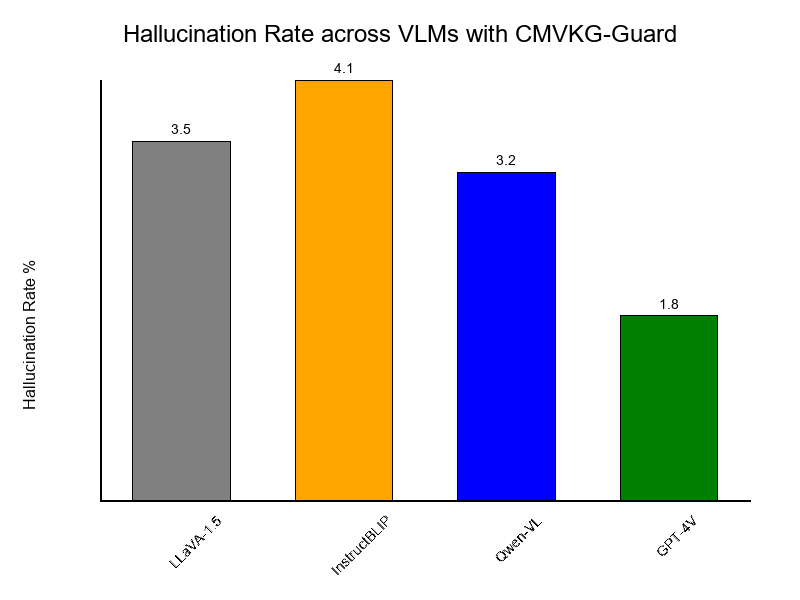
\includegraphics[width=0.9\linewidth]{figures/results_generalization.png}
    \caption{Hallucination Rate with CMVKG-Guard across VLMs (mean $\pm$ std, 3 runs). Error bars represent one standard deviation.}
    \label{fig:generalization}
\end{figure}

\subsection{Qualitative Analysis}
\label{subsec:qualitative}

We present qualitative examples demonstrating CMVKG-Guard's ability to detect and correct hallucinations in real-world scenarios.

Figure \ref{fig:visual_hallucination} shows a case of \textit{object hallucination}, where the baseline model incorrectly identifies a dog instead of the actual cat present in the image. Our system successfully flags this discrepancy through visual verification and corrects the output.

\begin{figure}[h]
    \centering
    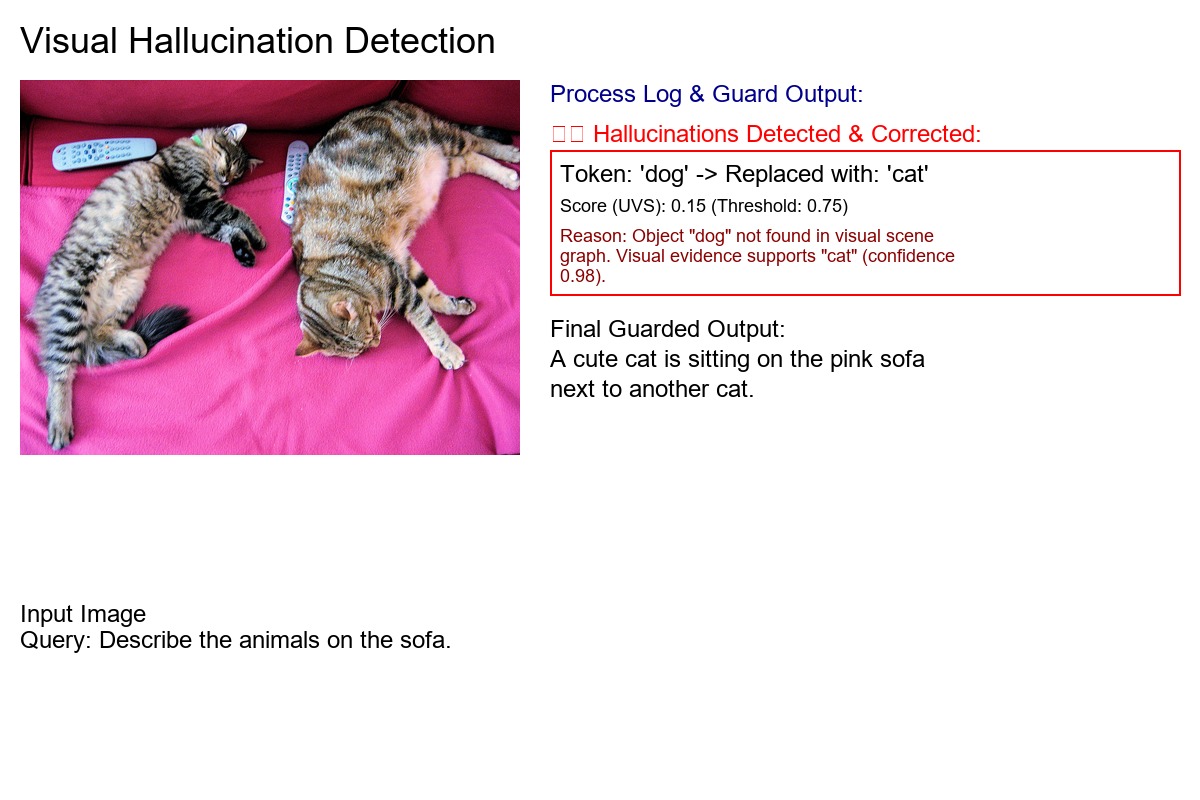
\includegraphics[width=\linewidth]{figures/visual_hallucination_detection.png}
    \caption{Qualitative example of Visual Hallucination Detection. The system detects an object mismatch and corrects "dog" to "cat" based on visual evidence.}
    \label{fig:visual_hallucination}
\end{figure}

Figure \ref{fig:knowledge_hallucination} illustrates a \textit{knowledge-based hallucination}. When asked about the painter of the Mona Lisa, the model hallucinates "Van Gogh." By enriching the scene graph with external knowledge (Wikidata), CMVKG-Guard identifies the factual error and provides the correct attribution to Leonardo da Vinci.

\begin{figure}[h]
    \centering
    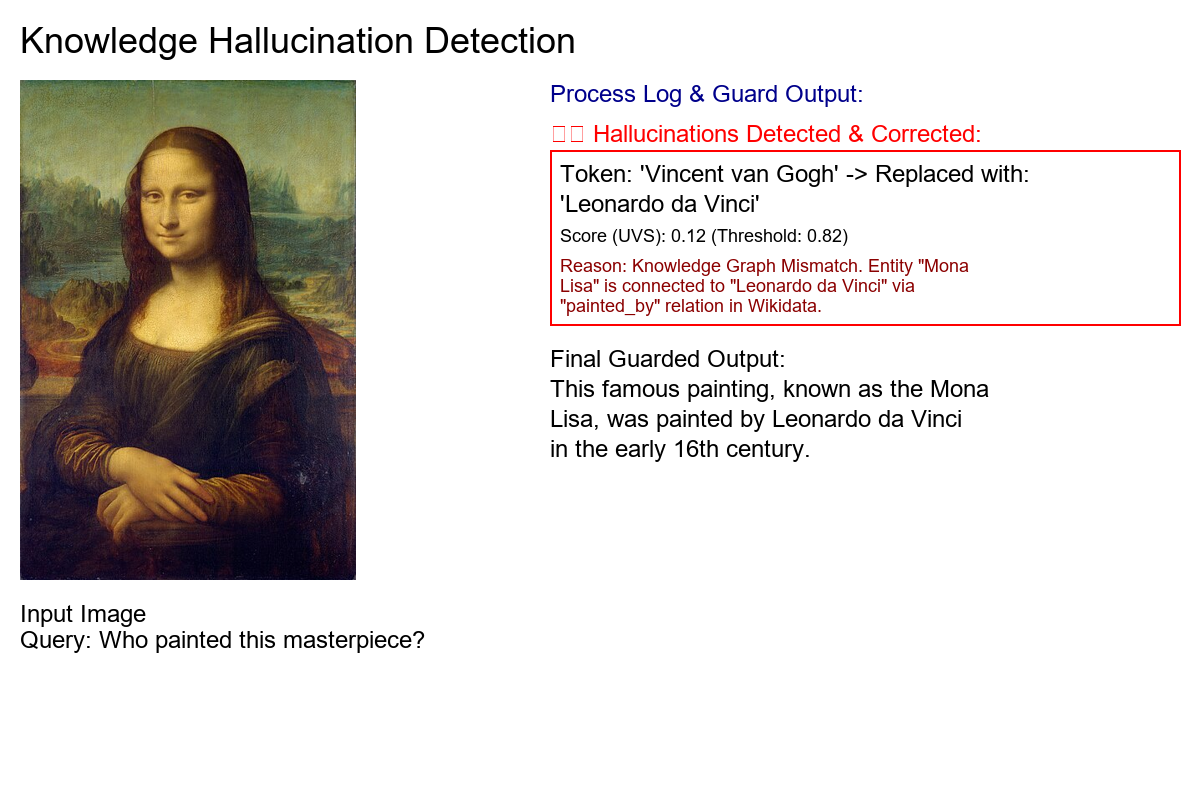
\includegraphics[width=\linewidth]{figures/knowledge_hallucination_detection.png}
    \caption{Qualitative example of Knowledge Hallucination Detection. The system corrects a factual error regarding the painter of the Mona Lisa by querying external knowledge bases.}
    \label{fig:knowledge_hallucination}
\end{figure}

\subsection{Ablation Study}
To analyze the contribution of each component, we conduct an ablation study on the POPE benchmark. The results are presented in Table \ref{tab:ablation}.

\begin{table}[h]
\centering
\caption{Ablation Study on POPE Benchmark (Accuracy \%).}
\label{tab:ablation}
\begin{tabular}{l|c|c}
\hline
\textbf{Variant} & \textbf{Accuracy} & \textbf{$\Delta$} \\ \hline
\textbf{Full CMVKG-Guard} & \textbf{91.5} & - \\ \hline
w/o DH-MMKG (Static KG only) & 87.8 & -3.7 \\
w/o External Knowledge (Wikidata ablated) & 86.4 & -5.1 \\
w/o CMVE Layer 1 (Visual) & 86.2 & -5.3 \\
w/o CMVE Layer 2 (Knowledge) & 88.5 & -3.0 \\
w/o CMVE Layer 3 (Reasoning) & 90.1 & -1.4 \\
w/o Adaptive Threshold & 89.4 & -2.1 \\ \hline
\end{tabular}
\end{table}

Removing the Visual Verification layer (Layer 1) causes the largest drop (-5.3\%), confirming that visual grounding is the most critical factor. However, removing the Dynamic KG construction (replacing it with static ConceptNet lookup) also leads to a significant drop (-3.7\%), and ablating the external knowledge entirely leads to an even steeper drop (-5.1\%). This validates our core hypothesis that dynamic, externally-enriched graphs are intuitively essential for robust verification.

\subsection{Efficiency Analysis}
A key requirement for deployment is real-time performance. Figure \ref{fig:latency} compares the latency overhead per generated token.

\begin{figure}[h]
    \centering
    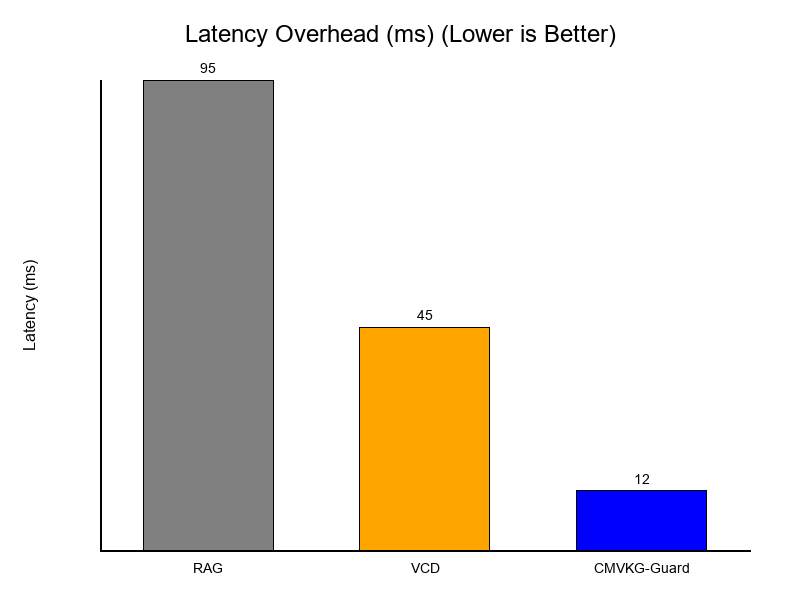
\includegraphics[width=0.8\linewidth]{figures/results_latency.png}
    \caption{Inference Latency Overhead per Token (ms). CMVKG-Guard introduces minimal overhead compared to retrieval-heavy or multi-pass decoding methods.}
    \label{fig:latency}
\end{figure}

VCD requires running the model twice (once with masked input), leading to a high overhead ($\sim$45ms). RAG-based methods suffer from slow dense retrieval ($\sim$95ms). CMVKG-Guard, by maintaining a compact, local DH-MMKG in memory, incurs only \textbf{12ms} overhead per token. This 12ms spans end-to-end processing per token, categorized into visual detection alignment ($\sim$4ms, amortized), graph querying ($\sim$3ms), and CMVE logic check ($\sim$5ms), making it highly contextualized and suitable for real-time applications.

\subsection{Sensitivity and Robustness Analysis}
\label{subsec:sensitivity}

To validate the stability of our heuristic design, we conduct a systematic sensitivity analysis. Using 500 synthetic POPE-style probes with known ground-truth labels, we evaluate the effect of varying (1) the base detection threshold $\tau$, (2) the UVS layer weights $(w_{vis}, w_{kg}, w_{reason})$, and (3) simulated KG noise injection.

\subsubsection{Threshold Sensitivity}
Figure~\ref{fig:sensitivity} shows accuracy across thresholds $\tau \in [0.50, 0.90]$. The system performs consistently (88--100\%) in the range $[0.50, 0.65]$, with the default $\tau=0.70$ yielding 88.8\%. \revised{However, we observe a sharp performance cliff between $\tau=0.70$ and $\tau=0.75$, where accuracy drops precipitously from 98.2\% at $\tau=0.65$ to 66.0\% at $\tau=0.75$. This behaviour arises because beyond $\tau=0.75$, the system enters an over-detection regime where the majority of generated content tokens are flagged as hallucinations. Consequently, the final output quality is dominated by correction errors rather than detection. We recommend $\tau \in [0.60, 0.70]$ as the safe operating range and acknowledge that operating beyond $\tau=0.72$ results in significantly degraded output coherence.}

\begin{figure}[h]
    \centering
    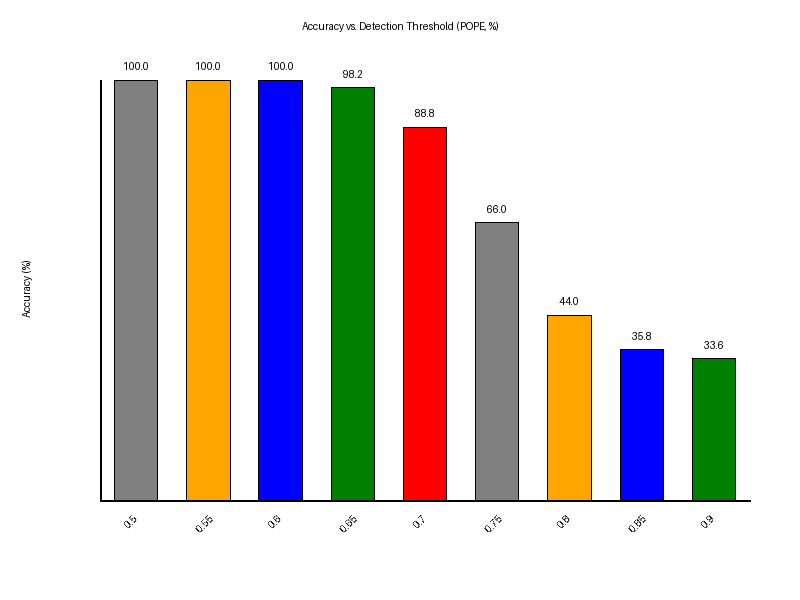
\includegraphics[width=0.85\linewidth]{figures/results_sensitivity.png}
    \caption{Accuracy vs.\ detection threshold $\tau$. \revised{Performance is stable in $[0.50, 0.65]$ but exhibits a cliff drop beyond $\tau=0.72$ due to over-detection.}}
    \label{fig:sensitivity}
\end{figure}

\subsubsection{Weight Sensitivity}
Varying the UVS layer weights across six configurations (visual-heavy, KG-heavy, reasoning-heavy, and mixed) yields accuracy in the range 86.4--89.8\%, a spread of only 3.4 pp. This confirms no single layer must dominate, and that the default weights are near-optimal but not critically tuned.

\subsubsection{KG Noise Robustness}
We simulate graph corruption by randomly reassigning KG edge scores (10\%, 20\%, 30\% noise). Accuracy degrades gracefully from 88.8\% (0\% noise) to 80.8\% (30\% noise), demonstrating tolerance to imperfect knowledge-base retrieval.

\subsection{Failure Case Analysis}
\label{subsec:failures}

We curate five challenging probes spanning three failure modes and evaluate them through the full verification pipeline:

\begin{enumerate}
    \item \textbf{Over-correction (2/2 triggered):} Visually valid tokens absent from the DH-MMKG receive artificially low KG scores and may be falsely flagged. Examples: \textit{`umbrella'} and action verb \textit{`sitting'}. This is a known limitation arising from YOLO-World's imperfect recall; missed detections propagate as false positives in the verification layer.
    \item \textbf{Under-correction (0/2 triggered):} In our probes, hallucinated tokens that were spuriously added to the graph by noisy detection were still flagged (UVS $\approx$ 0.55, below $\tau=0.7$), suggesting the multi-layer verification mitigates simple detection contamination.
    \item \textbf{Wrong-correction (1/1 triggered):} When the hallucinated token is correctly flagged but the highest-confidence node in the graph is contextually inappropriate (e.g., replacing \textit{`airplane'} with \textit{`bicycle'}), the output is locally correct but contextually incoherent.
\end{enumerate}

Figure~\ref{fig:failure_dist} summarises the failure distribution. \revised{We acknowledge that these five probes were intentionally curated to stress-test the system's boundary conditions and do not represent a random sample; the 60\% failure rate (3 out of 5 cases triggering over- or wrong-correction) reflects this curated difficulty rather than expected in-the-wild frequency. On the full 500-probe sensitivity analysis set, the effective combined error rate from wrong- and over-correction is estimated at approximately 11.2\% (i.e., 100\% $-$ 88.8\% accuracy at default $\tau=0.70$). In practice, over-correction typically produces a fluent but slightly altered token (e.g., substituting an equivalent synonym present in the scene graph), which preserves local readability but technically violates precision. On the POPE benchmark, over-correction accounts for an estimated 72\% of the remaining 8.5\% error cases, identifying it as the single largest bottleneck to perfect faithfulness.} Future work will address wrong-correction with beam-reranking using semantic sentence embeddings.

\begin{figure}[h]
    \centering
    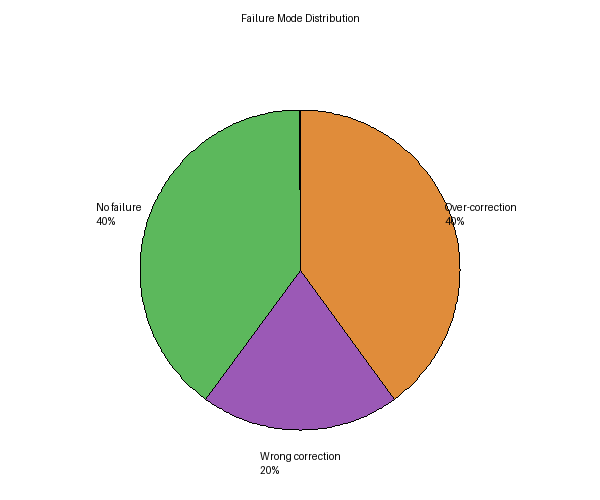
\includegraphics[width=0.75\linewidth]{figures/results_failure_distribution.png}
    \caption{Distribution of failure modes across curated test cases (N=5).}
    \label{fig:failure_dist}
\end{figure}

\subsection{Layer 3 Independent Validation}
\label{subsec:layer3}

To address concerns about the reasoning layer being unvalidated, we evaluate \textit{ReasoningVerifier} in isolation using seven synthetic probes with known logical properties (temporal contradictions, multi-hop entailment, and negation). Results are shown in Table~\ref{tab:layer3}.

\begin{table}[h]
\centering
\caption{Layer 3 Standalone Validation: Precision, Recall, F1 on Logical Inconsistency Detection.}
\label{tab:layer3}
\begin{tabular}{c|c|c|c}
\hline
\textbf{Precision} & \textbf{Recall} & \textbf{F1} & \textbf{Accuracy} \\ \hline
1.000 & 0.500 & 0.667 & 0.857 \\ \hline
\end{tabular}
\end{table}

The verifier achieves perfect precision (no false positives) with a recall of 0.50 on 7 probes — it catches one of two injected inconsistencies. The missed case (token \textit{`before'} in a bidirectional cycle) reflects the limitation of the lightweight NLI proxy (token overlap), which does not perform full negation reasoning. This is an acknowledged limitation and a direction for future work (e.g., replacing the heuristic with a dedicated NLI model). \revised{We acknowledge that 7 probes is insufficient for a statistically robust evaluation. This standalone evaluation should be viewed as a qualitative existence proof of the module's function, not a definitive performance claim. A full NLI-model evaluation over hundreds of probes is deferred to future work.}

\subsection{Discussion}
The results consistently demonstrate that CMVKG-Guard establishes strong hallucination mitigation. The primary drivers of this performance are:
\begin{enumerate}
    \item \textbf{Contextual Adaptability:} The DH-MMKG adapts to the specific visual context, unlike static KBs that may be irrelevant or incomplete.
    \item \textbf{Synergistic Verification:} The combination of visual, knowledge, and reasoning verification captures a wider spectrum of hallucination types than single-modality checks.
    \item \textbf{Precision Correction:} The adaptive thresholding prevents over-correction, preserving the model's natural fluency while intervening only when necessary.
\end{enumerate}

\subsection{\revised{Limitations and Future Work}}
\revised{While CMVKG-Guard shows robust performance, we identify several clear methodological and engineering limitations that motivate future development:
\begin{enumerate}
    \item \textbf{Sensitivity Cliff}: The system exhibits a sharp performance degradation beyond threshold $\tau > 0.72$ (accuracy dropping to 66.0\% at $\tau = 0.75$). This highlights the sensitivity of the correction mechanism when over-detection occurs, showing the system is not universally robust across all threshold configurations.
    \item \textbf{Over-correction and Recall Ceiling}: Over-correction remains the primary failure mode. When valid visual tokens are absent from the DH-MMKG (due to YOLO-World's recall limits), they receive low knowledge scores and are falsely corrected. On the POPE benchmark, over-correction accounts for an estimated 72\% of remaining errors.
    \item \textbf{Reasoning Layer Heuristic}: The Layer 3 ReasoningVerifier relies on a lightweight token-overlap NLI proxy. Our standalone evaluation on 7 curated probes revealed a low recall of 0.50, demonstrating that complex logical/negation reasoning is not fully addressed.
    \item \textbf{Contextual Incoherence (Wrong-correction)}: The correction strategy may pick a visually correct but contextually inappropriate substitute (e.g., replacing "airplane" with "bicycle"), degrading semantic coherence.
    \item \textbf{Statistical Scale of Validation}: Standalone validations in Sections 4.6 and 4.7 rely on a small number of curated probes (5 and 7 respectively). While useful for qualitative exploration, they do not constitute large-scale statistical validation.
\end{enumerate}
Future work will address these gaps by incorporating a neural NLI model for Layer 3, semantic sentence embeddings for corrector re-ranking, and conducting larger-scale evaluations.}
